\documentclass[11pt]{article}
\usepackage{amsmath,amsthm,amssymb,fullpage,graphicx,hyperref,listings}
\usepackage{listings,color,setspace}
\author{Andy Reagan}
\title{Math 337 Homework 14}

     \def\NN{\mathbb{N} }
     \def\ZZ{\mathbb{Z} }
     \def\QQ{\mathbb{Q} }
     \def\RR{\mathbb{R} }
     \def\CC{\mathbb{C} }
     \def\f{\frac }
     \def\b{\begin }
     \def\e{\end }
     \def\Log{\text{Log} \,}
     \def\Re{\text{Re} \, }
     \newcommand{\pdiff}[2]{\frac{\partial #1}{\partial #2}}
     \newcommand{\partialdiff}[2]{\frac{\partial #1}{\partial #2}}
     \newcommand{\pdiffsq}[2]{\frac{\partial^2 #1}{{\partial #2}^2}}
     \newcommand{\pdiffcu}[2]{\frac{\partial^3 #1}{{\partial #2}^3}}
     \newcommand{\pdiffhi}[3]{\frac{\partial^#3 #1}{{\partial #2}^#3}}
     \newcommand{\diff}[2]{\frac{{\rm d}#1}{{\rm d}#2}}
     \newcommand{\diffsq}[2]{\frac{{\rm d}^{2}#1}{{\rm d} {#2}^2}}
     \newcommand{\diffhi}[3]{\frac{{\rm d}^#3 #1}{{\rm d} {#2}^#3}}
     \newcommand{\tdiff}[2]{\mbox{d} #1/\mbox{d} #2}
     \newcommand{\tdiffsq}[2]{\mbox{d}^{2} #1/\mbox{d} {#2}^2}
     \newcommand{\tpdiff}[2]{\partial #1/\partial #2}
     \newcommand{\tpdiffsq}[2]{\partial^2 #1/\partial {#2}^2}
     \newcommand{\bvec}[1]{\vec{ {\bf #1 } }}
     \newcommand{\oh}[1]{O(h^{{#1}})}

\lstset{language=MATLAB,
basicstyle=\ttfamily\scriptsize\singlespacing,
keywordstyle=\color{black},
stringstyle=\color{black},
commentstyle=\color{black},
morecomment=[l][\color{black}]{\#},
frame=L,
xleftmargin=\parindent,
%%numbers=left,                   %% where to put the line-numbers
%%numberstyle=\scriptsize,      %% the size of the fonts that are used for the line-numbers
%%stepnumber=1,                   %% the step between two line-numbers. If it is 1 each line will be numbered
numbersep=5pt,
breaklines=true,        %% sets automatic line breaking
breakatwhitespace=false,    %% sets if automatic breaks should only happen at whitespace
escapeinside={\%*}{*)} 
}

%% example code insert
%% \lstinputlisting[language=Matlab]{andy_hw12_prb01.m}

%% example figure
%% \begin{figure}[h!]
%%   \centering
%%     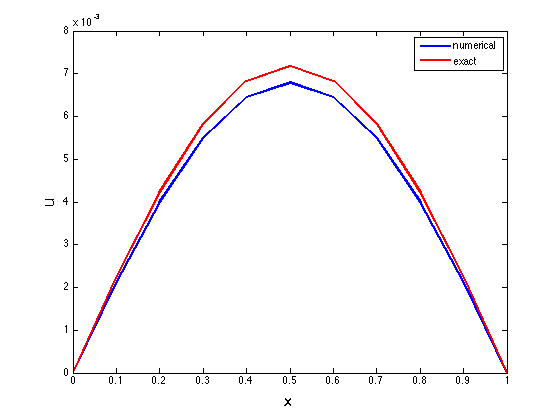
\includegraphics[width=0.45\textwidth]{andy_hw12_prb01_02.png}
%%   \caption{The numerical and exact solution for $h=0.1$.}
%% \end{figure}

%% start problem on next page
%% \clearpage
%% \pagebreak

\begin{document}
\maketitle

\begin{enumerate}

\item I solve the IBVP using method (14.10). To check the $u_x$ boundary condition is verified, we approximate
\begin{align*} u'_0 &= \f{u_1-u_0}{h} - \f{h}{2} u_0 '' + \oh{2}\\
&= \f{u_1-u_0}{h} -  \f{h}{2} \left ( \f{u_2 -2u_1 +u_0}{h^2} + \oh{1} \right ) + \oh{2}\\
&= \f{u_1-u_0}{h} -  \f{u_2 -2u_1 +u_0}{2h} + \oh{2} .\end{align*}

In addition to the solution at time $t=2$, I include a plot of the error in the numerical solution BC at $x = 0$, the mixed BC.

\lstinputlisting[language=Matlab]{andy_hw14_prb01.m}

\begin{figure}[h!]
  \centering
    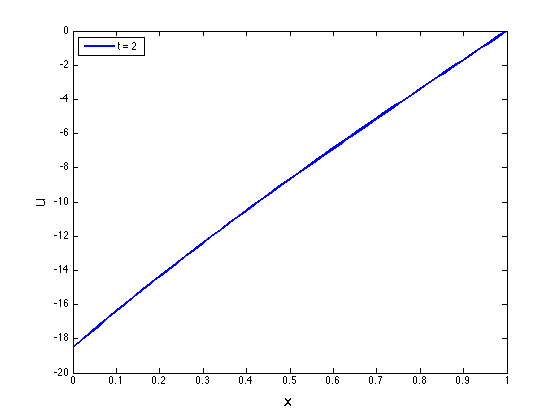
\includegraphics[width=0.45\textwidth]{andy_hw14_prb01_01.png}
  \caption{Solution of IBVP of Problem 1 using method 14.12.}
\end{figure}

\begin{figure}[h!]
  \centering
    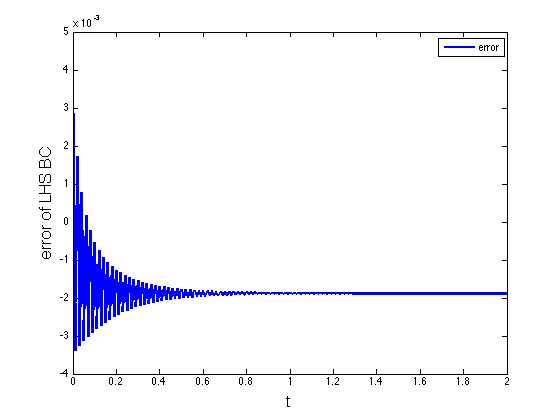
\includegraphics[width=0.45\textwidth]{andy_hw14_prb01_03.png}
  \caption{Error in the BC at $x=0$ of the numerical solution of IBVP of Problem 1 using method 14.12.}
\end{figure}

Bonus (i): I make an attempt, although I do not think this is complete.

Substituting the form $u(x,t)$ into the PDE, we have
\[ \lambda e ^{\lambda t} \left ( A e ^{kx} + B e ^{-kx} \right ) = k^2 e ^{\lambda t} \left ( A e ^{kx} + B e ^{-kx} \right ) \]
Clearly, this gives us the condition that $\lambda = k^2$.

Now we find $A$ and $B$ from the BC.
First for the RHS BC:
\begin{align*} e ^{\lambda t} \left ( A e ^{k} + B e ^{-k} \right ) & = 0\\
A e ^{k} + B e ^{-k} & = 0\\
A e ^{k} &= - B e ^{-k} \\
A &= - B e ^{-2k} \end{align*}

Now for the LHS (mixed) BC (the exponentials are eqaul to 1 at $x=0$, and this is homogeneous so the RHS is 0):
\begin{align*} e ^{\lambda t} \left ( kA  - kB \right ) + p e ^{\lambda t} \left ( A +B \right )& = 0\\
k\left ( A  - B \right ) + p \left ( A +B \right )& = 0\\
k\left ( - B e ^{-2k}  - B\right ) + p \left ( - B e ^{-2k} +B \right )& = 0\\
kB\left ( - e ^{-2k}  - 1\right ) + p B \left ( - e ^{-2k} + 1 \right )& = 0\end{align*}

Now we need to decide what it is that we are solving for, since we have two free parameters $k$ and $B$.
I am unsure how to proceed, (of course we can obtain a more concise form for all three parameters) but for the purposes of this problem I let $B$ be arbitrary and we have
\begin{align*} k\left ( - e ^{-2k}  - 1\right ) + p \left ( - e ^{-2k} + 1 \right )& = 0\\
k\f{ 1 + e ^{-2k}  } { 1 - e ^{-2k} } &= p \end{align*}

Plotting $p$ versus real $k$ we see that for $p=1$ the only solution is $k=0$, and for $p>1$ there are always two solutions.
For $p<1$, there are clearly no real solutions.
So, for $p>1$, we have that $k$ is real and since $\lambda = k^2$, we will have unbounded growth of the analytical solution.

More specifically, the term $e^{\lambda t} = e^{k^2 t}$ will grow exponentially as $t$ increases, such that any solution will be unstable.
Here, since $B$ was arbitrary, this holds for any $B$ we could have chosen.

\begin{figure}[h!]
  \centering
    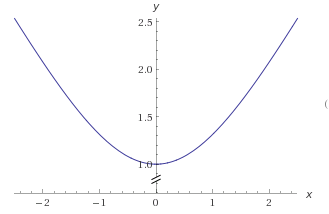
\includegraphics[width=0.45\textwidth]{andy_hw14_prb01i_01.png}
  \caption{A plot of the magnitude of $p$ versus real $k$.}
\end{figure}

Bonus (ii): Let $p,q$ be constant and define $v(x,t) = u(x,t) + \f{q}{p-1}(x -1)$.
The partial derivatives of $v_{xx},v_t$ are the same as $u_{xx},u_t$, so this $v$ also satisfies the heat equation.
At the RHS, where $x=1$, the term that we've added is clearly 0.
Finally, observe that
\[ v_x (0,t) + p v (0,t) = u_x(0,t) + \f{q}{p - 1} + p u(0,t) - \f{p q}{p - 1} = u_x(0,t) + p u(0,t) + \f{q-pq}{p - 1}  = u_x(0,t) + p u(0,t) -q .\]
such that for homogenous $v$, it satifies the equation for the inhomogeneous $u$.

This explains the result for $p<1$ because we're substracting a multiple of $x-1$ from our solution, so it is greater than for $p=1$.

\begin{figure}[h!]
  \centering
    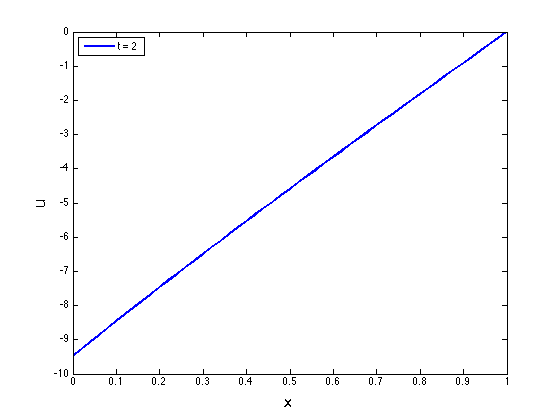
\includegraphics[width=0.45\textwidth]{andy_hw14_prb01ii_01.png}
  \caption{Solution of IBVP of Problem 1 with $p=0.75$.
    We observe that the solution is less negative than for $p=1$, owing to the effective transformation to a new problem where we have subtracted a multiple of $x-1$ from the solution.}
\end{figure}


\clearpage
\pagebreak
\item The numerical scheme (14.19), upon plugging in for $\delta _x ^2$ and $\delta _t$ becomes (gathering terms in $U_i ^j$, and letting $\gamma = 1$):
\begin{align*} &U_{m+1} ^{n+1} \left ( -\f{r}{2} \alpha _{m+1/2} ^{n+1} +\f{r}{2} \alpha _{m-1/2} ^{n+1} \right ) + U_{m} ^{n+1} \left ( 1 - \f{\kappa}{2} \beta _{m} ^{n+1} +r \alpha _{m+1/2} ^{n+1} -r \alpha _{m-1/2} ^{n+1} \right )\\
&~~~~ + U_{m+1} ^{n+1} \left ( \f{r}{2} \alpha _{m+1/2} ^{n+1} -\f{r}{2} \alpha _{m-1/2} ^{n+1} \right )\\
&~~~~ = U_{m+1} ^{n} \left ( \f{r}{2} \alpha _{m+1/2} ^{n} -\f{r}{2} \alpha _{m-1/2} ^{n} \right ) + U_{m} ^{n} \left ( 1 + \f{\kappa}{2} \beta _{m} ^{n} -r \alpha _{m+1/2} ^{n} +r \alpha _{m-1/2} ^{n} \right )\\
&~~~~ + U_{m+1} ^{n} \left ( - \f{r}{2} \alpha _{m+1/2} ^{n} +\f{r}{2} \alpha _{m-1/2} ^{n} \right )\end{align*}

\lstinputlisting[language=Matlab]{andy_hw14_prb02.m}

\begin{figure}[h!]
  \centering
    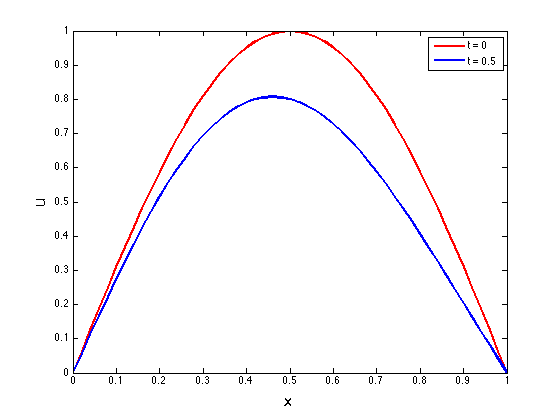
\includegraphics[width=0.45\textwidth]{andy_hw14_prb02_01.png}
  \caption{Solution of IBVP of Problem 2 using method 14.19.}
\end{figure}

\clearpage
\pagebreak
\item Applying the Von Nuemann stability analysis, we have
\[ \f{U_{m+1} ^{n+1}-2U_{m} ^{n+1}+U_{m-1} ^{n+1}}{h^2} = \f{3}{2} \f{U_{m} ^{n+1}-U_{m} ^{n}}{\kappa} - \f{1}{2} \f{U_{m} ^{n} - U_{m} ^{n-1}}{\kappa}. \]
Letting $r = \kappa/h^2$, 
\[ 2r \left ( U_{m+1} ^{n+1}-2U_{m} ^{n+1}+U_{m-1} ^{n+1}\right )  = 3\left ( U_{m} ^{n+1}-U_{m} ^{n} \right )  + \left ( U_{m} ^{n} - U_{m} ^{n-1} \right ), \]
and since this in linear, we replace $U$ with the error $\epsilon$ 
\[ 2r \left (\epsilon_{m+1} ^{n+1}-2\epsilon_{m} ^{n+1}+\epsilon_{m-1} ^{n+1}\right )  = 3\left ( \epsilon_{m} ^{n+1}-\epsilon_{m} ^{n} \right )  - \left ( \epsilon_{m} ^{n} - \epsilon_{m} ^{n-1} \right ), \]
Now we expand $\epsilon$ with a specific Fourier series, namely $\epsilon \to \rho ^n e^{i\beta m h}$:
\begin{align*} 2r \left (\rho ^{n+1} e ^{i \beta (m+1) h}-2\rho ^{n+1} e ^{i \beta (m) h}+\rho ^{n+1} e ^{i \beta (m-1) h}\right )  &= 3\left ( \rho ^{n+1} e ^{i \beta (m) h}-\rho ^{n} e ^{i \beta (m) h}\right ) \\
&~~~~- \left ( \rho ^{n} e ^{i \beta (m) h} - \rho ^{n-1} e ^{i \beta (m) h} \right ). \end{align*}
Cancelling $\rho ^{n-1} e^{i\beta m h}$, we are left
\begin{align*} 2r \left (\rho ^{2} e ^{i \beta h}-2\rho ^{2} +\rho ^{2} e ^{-i \beta }\right )  = 3\left ( \rho ^{2} -\rho \right )- \left ( \rho - 1\right ). \end{align*}
Finally, I collect the remaining exponentials in to a cosine term, and we have
\begin{align*} 4r\rho ^{2} \left ( \cos (\beta h)-1\right )  = 3\rho \left ( \rho -1\right )- \left ( \rho - 1\right ) = 3\rho ^2 -4\rho +1 . \end{align*}
Which is
\begin{align*} 4r\rho ^{2} \left ( \cos (\beta h)-1\right )  - 3\rho ^2 +4\rho -1  = 0. \end{align*}
Although we could simplify this and plot in 2D, it is simpler just to look at the magnitude of $\rho$ versus a reasonable range of $r$ and $\beta h$ independently.
Now we turn to plotting the largest magnitude root $\rho$ for $\beta h \in [0,\pi]$ and $r \in [0,10]$.
The following code does just that:

\lstinputlisting[language=Matlab]{andy_hw14_prb03.m}

\begin{figure}[t!]
  \centering
    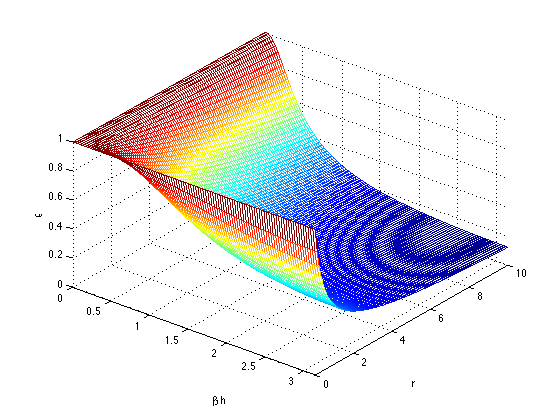
\includegraphics[width=0.45\textwidth]{andy_hw14_prb03_01.png}
  \caption{Magnitude of the largest root $\rho$ in the Von Nuemann stability analysis of the scheme of Problem 3.
  We observe unconditional stability, since the largest root $\rho$ has magnitude less than one for $\beta h \ne 0, r\ne 0$.}
\end{figure}

It appears that this method will better smooth a discontinuous initial condition, since for $\beta h$ close to 0, (the highest frequency mode), this method has $\rho$ drop off more quickly than the CN method.

\clearpage
\pagebreak
\item To solve the nonlinear IBVP, I first attempt using the semi-implicit method described by Eq. 14.50 of the notes.
The main reason that I attempt this first is that the Newton-Raphson looks cumbersome to code.

To resolve both the IC and final solution, I set $h=.02$.
I include a plot of the the initial and final solution, the final solution and asymptotically exact, the error versus x, and the max error versus time.

\lstinputlisting[language=Matlab]{andy_hw14_prb04.m}

\begin{figure}[t!]
  \centering
    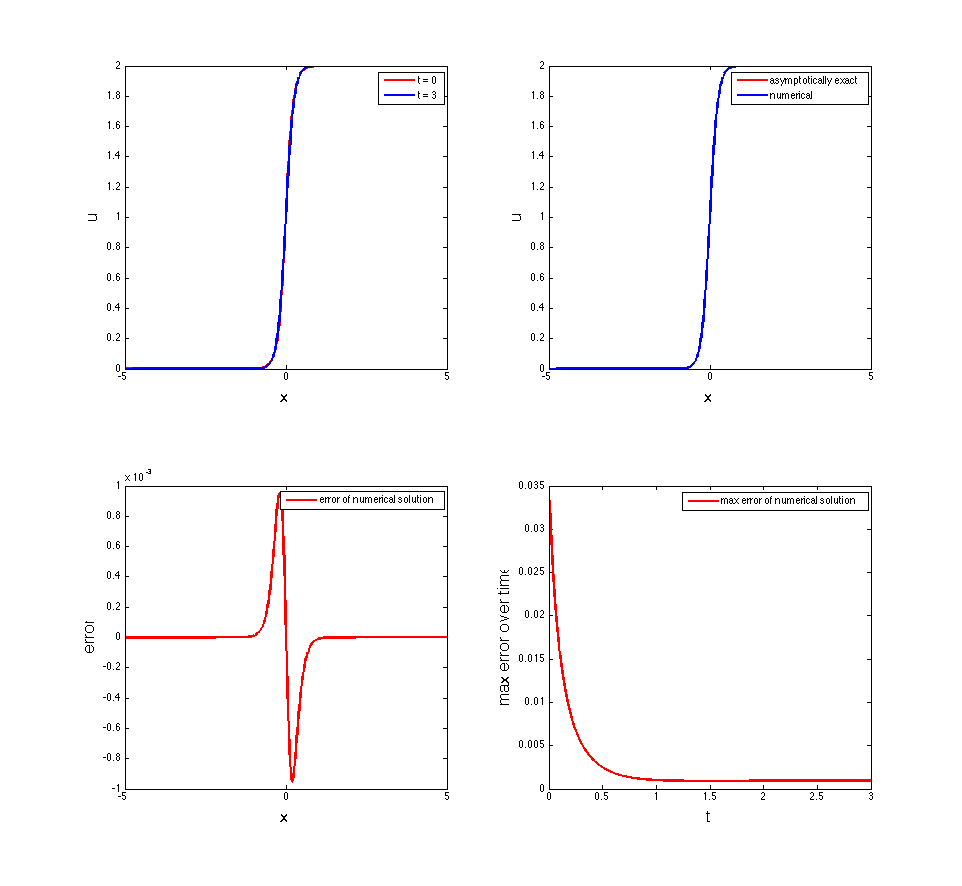
\includegraphics[width=0.45\textwidth]{andy_hw14_prb04_g01_01.png}
  \caption{Here $\gamma = 0.125$. I include a plot of the the initial and final solution, the final solution and asymptotically exact, the error versus x, and the max error versus time.
  The plot versus time is to see that we are approaching the exact solution, which is exact in the asymtotic limit.}
\end{figure}

\begin{figure}[t!]
  \centering
    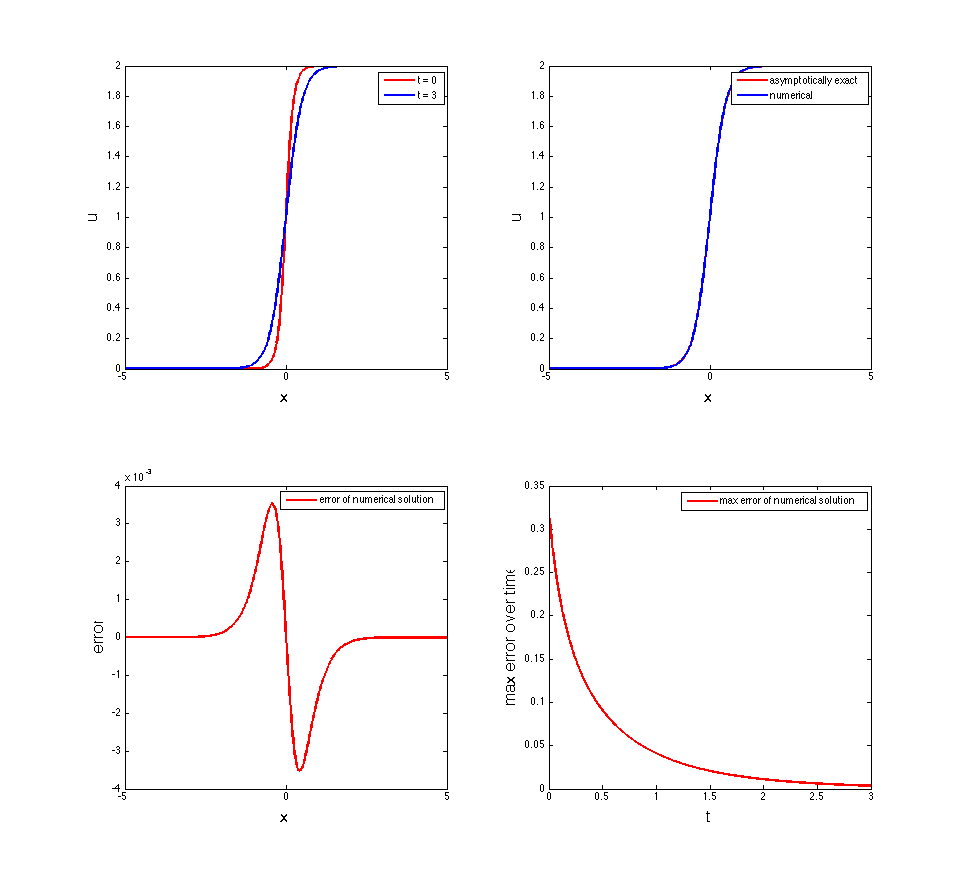
\includegraphics[width=0.45\textwidth]{andy_hw14_prb04_g02_01.png}
  \caption{Here $\gamma = 0.25$. I include a plot of the the initial and final solution, the final solution and asymptotically exact, the error versus x, and the max error versus time.
  The plot versus time is to see that we are approaching the exact solution, which is exact in the asymtotic limit.}
\end{figure}

\begin{figure}[t!]
  \centering
    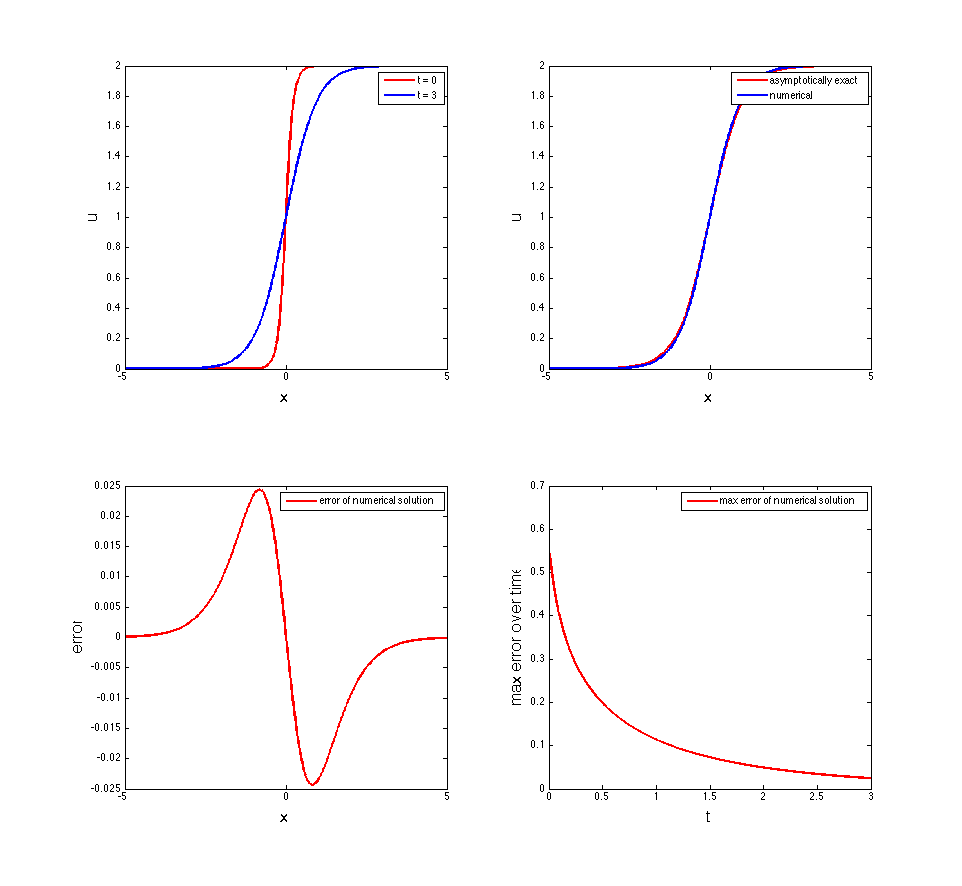
\includegraphics[width=0.45\textwidth]{andy_hw14_prb04_g03_01.png}
  \caption{Here $\gamma = 0.5$. I include a plot of the the initial and final solution, the final solution and asymptotically exact, the error versus x, and the max error versus time.
  The plot versus time is to see that we are approaching the exact solution, which is exact in the asymtotic limit.}
\end{figure}




\end{enumerate}
\end{document}



